\documentclass{article}

\usepackage{graphicx}

\graphicspath{./}
    
\begin{document}
    \title  { \textbf{SYSC 4602 Assignment 1} }
    \author {
        David Song (101071234)\\
        Ghassan Arnouk (101078550)\\
        Zachary Porter (101069001)
    }
     
    \maketitle
    
    \clearpage
    \section*{Part 3: Ethernet Frame Structure}
    \begin{figure}[htbp]
        \centering
        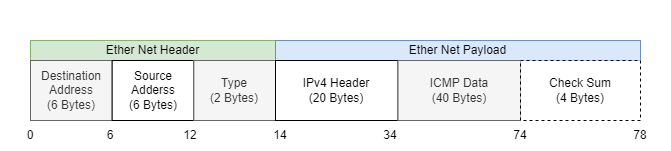
\includegraphics[width=\textwidth]{images/assignment3-part3.drawio.png}
        \caption{Ethernet Frame Structure Diagram}
    \end{figure}
    \section*{Part 4: Protocol Overhead}
    \begin{figure}[htbp]
        \centering
        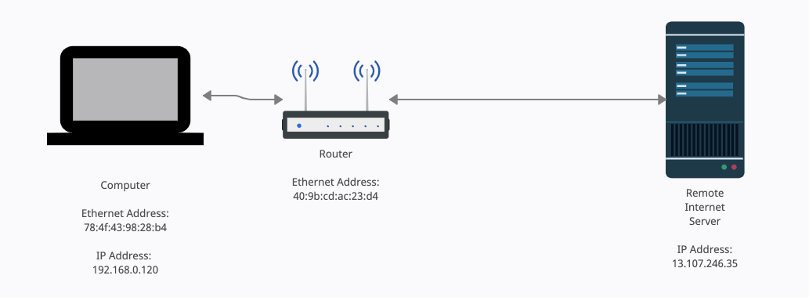
\includegraphics[width=\linewidth]{images/part4.png}
        \caption{Relative positions of computer, router, and internet server}
    \end{figure}
    \section*{Part 5: Demultiplexing Keys}
    \subsection*{What is the broadcast Ethernet address, written standard form as Wireshark displays it?}
    The broadcast ethernet address is {\bfseries FF FF FF FF FF FF} which is represented as all {\bfseries 1's} in hexadecimal.
    As stated in the lab manual, broadcast traffic is sent to a reserved Ethernet address that has all bits set to {\bfseries 1's}.
    \clearpage
    \subsection*{Which bit of the Ethernet address is used to determine whether it is unicast or multicast/broadcast?}
    The ethernet address uses the {\bfseries first bit} to determine whether it is unicast or multicast/broadcast.
    If the first bit is `0', it is denoted as unicast, whereas if it's `1', it is denoted as multicast/broadcast. 
    Note that broadcast is a special case of multicast and thus; they are both denoted using the first bit as `1'.
\end{document}
